\documentclass{JNUexp}
\courseName{Linux 环境程序设计}
\expName{实验 6 Linux 环境编程}
\expDate{2017.11.29}
\className{计科1404}
\studentName{阎覃}
\studentId{1030414414}

\graphicspath{ {images/} }

\usepackage[hidelinks]{hyperref}
\begin{document} 

\section{实验目的}
\begin{itemize}
    \item 理解系统调用和库函数的异同;
    \item 学会用系统调用进行编程;
    \item 掌握一些常用的系统调用的功能及应用。
\end{itemize}

\section{实验内容}
\begin{itemize}
    \item 使用系统调用对文件进行操作;
    \item 使用系统调用对进程进行控制;
    \item 使用管道机制进行 I/O;
    \item 使用信号机制进行进程通信。
\end{itemize}
\section{实验步骤及运行情况}
%%%%%%%%%%%%%%%%%%%%%%%%%%%%%%%%%%%%%%%%%%%%%%%%%%%%%%%%%
%   1
%%%%%%%%%%%%%%%%%%%%%%%%%%%%%%%%%%%%%%%%%%%%%%%%%%%%%%%%%
\begin{problem}
    编写一个程序,把一个文件的内容复制到另一个文件上,即实现简单的 copy 功能。要求:
    只用 open(),read(),write()和 close()系统调用,程序的第一个参数是 源文件,
    第二个参数是目的文件。
\end{problem}

\begin{answer}
    下面是程序的源代码:
    \lstinputlisting[language={[11]C++}]{../src/copy/main.cpp}
\end{answer}

\begin{image}
    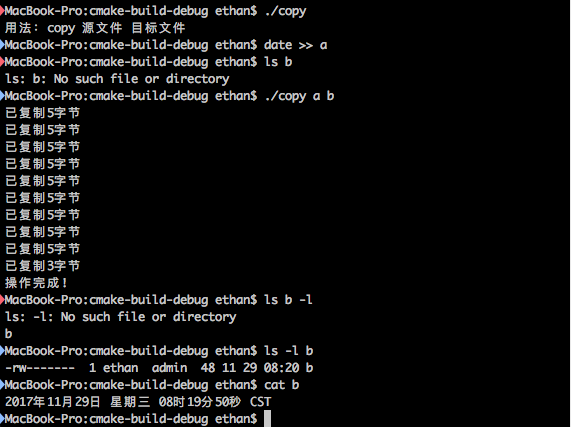
\includegraphics[width=0.7\textwidth]{1}
\end{image}
%%%%%%%%%%%%%%%%%%%%%%%%%%%%%%%%%%%%%%%%%%%%%%%%%%%%%%%%%
%   2
%%%%%%%%%%%%%%%%%%%%%%%%%%%%%%%%%%%%%%%%%%%%%%%%%%%%%%%%%
\begin{problem}
    编写一个程序,它利用 fork()创建一个子进程;父进程打开一个文件, 父子进程都向文件
    写入(利用 write())信息,表明是在哪个进程中;每个进程都打印两个进 程的 ID 号。最
    后父进程执行 wait()。另外,如果没有 wait 调用,会出现什么情况?
\end{problem}

\begin{answer}
    下面是程序的源代码:
    \lstinputlisting[language={[11]C++}]{../src/fork/main.cpp}
    如果没有wait调用,子进程将会成为僵死进程。
\end{answer}

\begin{image}
    
\includegraphics[width=0.7\textwidth]{2}
\end{image}
%%%%%%%%%%%%%%%%%%%%%%%%%%%%%%%%%%%%%%%%%%%%%%%%%%%%%%%%%
%   3
%%%%%%%%%%%%%%%%%%%%%%%%%%%%%%%%%%%%%%%%%%%%%%%%%%%%%%%%%
\begin{problem}
    编写一个程序,它创建一个子进程。父进程向子进程发送一个信号,然 后等待子进程终止;子
    进程接受信号,输出自己的状态信息,最后终止自己。
\end{problem}

\begin{answer}
    下面是程序的源代码:
    \lstinputlisting[language={[11]C++}]{../src/signal/main.cpp}

\end{answer}

\begin{image}
    
\includegraphics[width=0.7\textwidth]{3}
\end{image}

%%%%%%%%%%%%%%%%%%%%%%%%%%%%%%%%%%%%%%%%%%%%%%%%%%%%%%%%%
%   4
%%%%%%%%%%%%%%%%%%%%%%%%%%%%%%%%%%%%%%%%%%%%%%%%%%%%%%%%%
\begin{problem}
    编译并运行教材 P220-221 例题 7.5,体会管道机制的应用。
\end{problem}

\begin{answer}
    下面是程序的源代码:
    \lstinputlisting[language={[11]C++}]{../src/pipe/main.cpp}
\end{answer}

\begin{image}
    
\includegraphics[width=0.7\textwidth]{4}
\end{image}
%%%%%%%%%%%%%%%%%%%%%%%%%%%%%%%%%%%%%%%%%%%%%%%%%%%%%%%%%
%   5
%%%%%%%%%%%%%%%%%%%%%%%%%%%%%%%%%%%%%%%%%%%%%%%%%%%%%%%%%
\begin{problem}
    掌握 Unix/Linux 环境下事件驱动编程的一般方法,能利用 curses 库、间隔计时器
    (interval timer)、信号处理编写一个功能完整的视频游 戏程序,并能在 Unix/Linux
    环境下正确地运行。
\end{problem}

\begin{answer}
    本游戏是一个躲避障碍的小游戏,用户可以按空格键操作小人,跳跃躲避障碍物。随着游戏的
    进行难度会不断提升。右上角会计分,当小人遇到障碍没有成功躲避时游戏结束。

    \lstinputlisting[language={[11]C++}]{../src/game/main.cpp}
\end{answer}

\begin{image}
    
\includegraphics[width=0.7\textwidth]{5}
\end{image}



\section{实验体会}
通过这次实验,我练习了许多Linux系统调用函数,同时也对一些系统调用得到了进一步的了解。包括
文件操作,进程间通信,定时,信号等等,都是Linux中的重要概念。最后的事件驱动编程编写了一个
完整的小游戏,提升了我的动手能力,并且增强了对Linux的兴趣。

\vfill

实验报告采用 \LaTeX 排版,代码托管至GitHub:\\
\url{https://github.com/Ethan-yt/JNU-Linux-exp}

\end{document}